\section{Aufbau und Durchführung}
Die Abbildung \ref{fig:aufbau} zeigt die schematische Darstellung der Messapparatur.  
Als Lichtquelle wird eine Halogen-Lampe verwendet, deren Emissionsspektrum hauptsächlich im infraroten Bereich liegt, da die Halbleiterprobe (Galliumarsenid) nur im Infrarot durchlässig ist. Der Strahl wird mit Hilfe einer Linse gebündelt und im Lichtzerhacker, rotierende Sektorscheibe, in Lichtimpulse umgewandelt. Anschließend trifft der Strahl auf ein Glan-Thompson-Prisma aus Kalkspalt und wird linear polarisiert. Zur Winkelmessung dient ein Goniometer, welches zwischen dem Prisma und dem Elektromagneten angebracht ist. Im Elektromagneten befindet sich in einem Luftspalt die Halbleiterprobe. Nachdem der Lichtstrahl die Probe passiert hat, filtert der Interferenzfilter einen bestimmten Wellenlängenbereich. Anschließend trifft das monochromatische Licht auf ein zweites Glan-Thompson Prisma, welches das Licht in zwei senkrecht zueinander polarisierte Strahlen teilt. Diese werden von zwei Photowiderständen aufgenommen. Dabei wird ein Spannungssignal erzeugt, welches von der Intensität des Lichtes abhängig ist. Aufgrund des hohen Innenwiderstandes in den Photowiderständen können Rauschspannungen entstehen. Deshalb wird mit der  Wechsellichtmethode gearbeitet, die durch den Lichtzerhacker gewährleistet ist. Die Wechselspannung am Photowiderstand wird mit Hilfe des Kondensators als zeitlich periodisches Licht gemessen und das Rauschen wird dabei herausgefiltert. Beide Signale der Photowiderstände werden zum Differenzverstärker geleitet. Dessen Ausgangsspannung ist proportional zur Differenz der Eingangsspannung und verschwindet dann, wenn beide Strahlen nach Betrag und Phase übereinstimmen. Anschließend wird das Ausgangssignal auf einen Selektivverstärker gegeben und am Oszilloskop, welches als Nulldetektor dient, angezeigt.

\begin{figure}[h!]
	\centering
	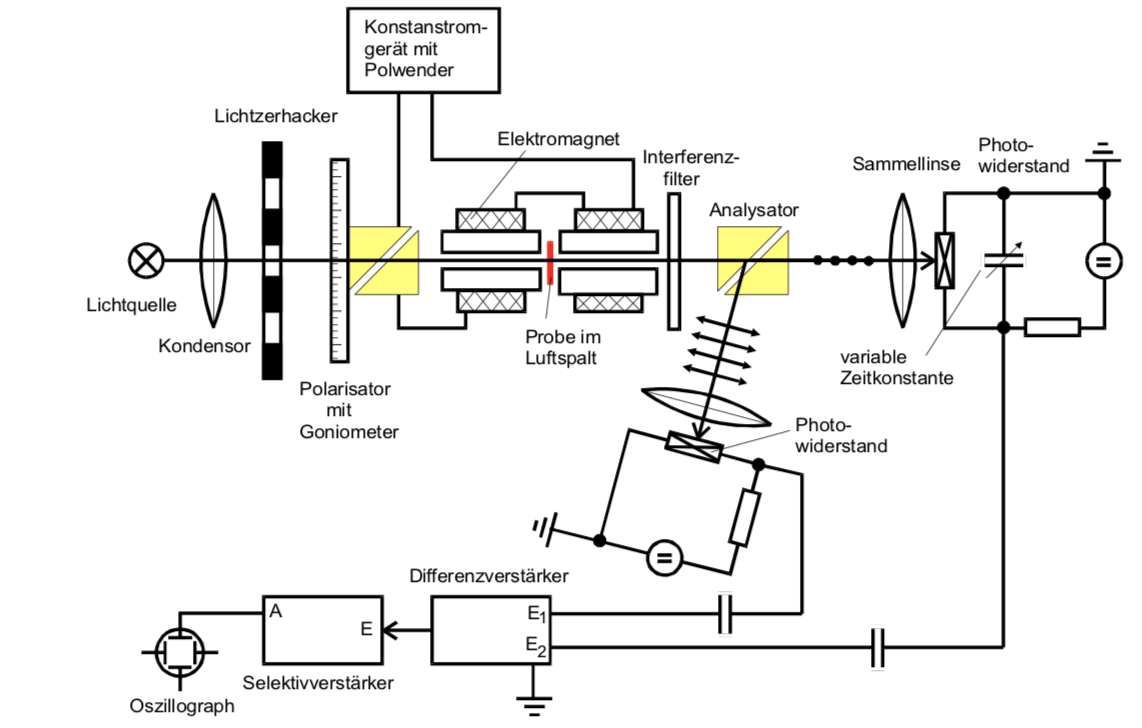
\includegraphics[width=0.8\linewidth]{../../Polina/aufbau}
	\caption{Versuchsapparatur, \cite{anleitungV46}.}
	\label{fig:aufbau}
\end{figure}

Bei der Durchführung werden die Winkel von zwei Halbleiterproben gemessen. Bei der Ersten handelt es sich um die hochreine Halbleiterprobe Galliumarsenid und bei der Zweiten um eine n-dotierte Galliumarsenid Probe (N=$1,2\cdot 10^{18}\text{cm}^{-3}$). Für jede Probe werden mehrere Interferenzfilter eingesetzt und die dazugehörigen Winkel gemessen.  Bei maximalem Magnetfeld kann das Prisma im Winkel verstellt und so lange variiert werden, bis der Spannungsunterschied an den Photowiderständen möglichst verschwindet. Dabei wird der erste Winkel $\theta_1$ bei dem der Spannungsunterschied am Oszilloskop verschwindet am Goniometer abgelesen. Anschließend wird das Magnetfeld umgepolt und der erste Schritt wiederholt. Der Winkel $\theta_2$ wird notiert. Der gesuchte Winkel wird mit Hilfe der Formel 
\begin{align}
\theta=\dfrac{1}{2}(\theta_1-\theta_2)
\end{align}
bestimmt. Um die Kraftflussdichte $B(z)$ entlang der Richtung des einfallenden Lichtes zu messen und die maximale Feldstärke zu bestimmen, wird eine Hallsonde im Magneten positioniert und für verschiedene Positionen die Feldstärke notiert. 
\subsection{Der Interferenzfilter}

Die Abbildung \ref{fig:interferenz} zeigt den schematischen Aufbau eines Interferenzfilters.

\begin{figure}[h!]
	\centering
	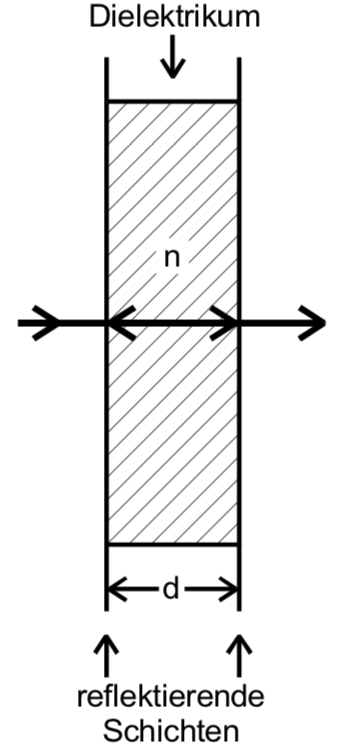
\includegraphics[width=0.2\linewidth]{../../Polina/interferenz}
	\caption{Querschnitt durch ein Interferenzfilter, \cite{anleitungV46}.}
	\label{fig:interferenz}
\end{figure}

Dieser besteht aus zwei reflektierenden Schichten und dazwischen ein Dielektrikum mit der Brechnungsindex $n$. Sobald ein Lichtstrahl auf den Filter trifft, wird es an der inneren Oberfläche mehrmals reflektiert. Dabei interferieren die Teilwellen. Konstruktive Interferenz entsteht für Licht welche die Bedingung 
\begin{align}
j\lambda_j=2nd+\lambda
\end{align}
erfüllen. 
\subsection{Das Glan-Thomson Prisma}
Die Abbildung \ref{fig:prisma} zeigt die Funktionsweise des Glan-Thomson Prismas. 

\begin{figure}[h!]
	\centering
	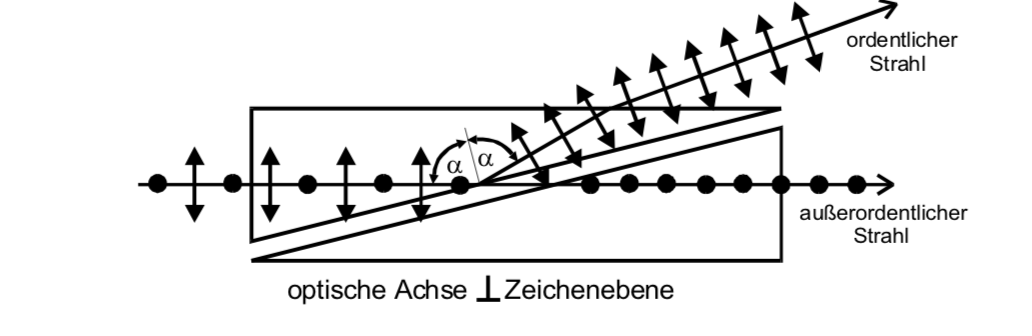
\includegraphics[width=0.9\linewidth]{../../Polina/prisma}
	\caption{Versuchsapparatur, \cite{anleitungV46}.}
	\label{fig:prisma}
\end{figure}

Es besteht aus zwei Prismen, die durch einen Luftschlitz von einander getrennt sind. Dies sorgt für eine Teilung des einfallenden Lichtstrahls in zwei senkrecht zueinander polarisierte Strahlen. Ermöglicht wird es dadurch, dass der einfallende Strahl an den Grenzflächen totalreflektiert wird, wenn das Verhältnis der Brechungsindizes 
\begin{align}
\dfrac{1}{n_0}<sin(\alpha)<\dfrac{1}{n_{ao}}
\end{align}
erfüllt ist. Hierbei ist $n_0$ der Brechungsindex des ordentlichen und $n_{ao}$ der Brechungsindex des außerordentlichen Strahls. 